\chapter{Prototype Evaluation Study}
\label{cha:evaluation}


\section{Introduction and Objectives}

We conducted an evaluation study of the prototype app in February 2019 with 6 forced migrants and 16 local freecyclers. The objective of the trial was to evaluate the usability and usefulness of the location-based freecycling service we developed in the second phase of the study, with respect to reducing the social isolation of forced migrants.

The independent variable in the study was the user group of the participant (forced migrant or experienced freecycler). The dependent variables that we tested were the reduction of social isolation (i.e., usefulness of the service) and the overall usability of service.

Having defined social isolation as the absence of social contact, we chose to measure reduction of social isolation simply by counting instances of contact with others that could be attributed to the functionality of the prototype service. Recognizing that relationships develop gradually with time, we decided to evaluate the creation of potential for deeper connections, instead of looking for changes in participants' social networks during the two weeks of the trial.

The study was randomized by allowing participants to self-select and by providing no restrictions or requirements for how participants used the app during the two-week trial period.


\section{Participants}

We recruited forced migrant participants by contacting participants from our first study and by reaching out to other forced migrants we had met during the course of the project. We attended forced migrant meet-ups and helped interested attendees install and sign up for the service in person. We additionally shared a request for participants in a WhatsApp group for forced migrants and other members of a local club for newcomers to Münster.

We recruited freecycling participants by posting in the two largest Münster freecycling platforms and by contacting participants from the first study who had expressed interest in later testing a prototype.

All participants lived in Münster and were 18 years old or older. We did not control for specific age or experience. We motivated participation with a 10 Euro reward, delivered at the end of the study.

Of the 29 people who downloaded the app and created an account during the trial, we approved 25 for the study. From that pool, 22 consented to participate, filled out all of the surveys, and saw the trial through to the very end. Six of these self-identified as forced migrants.

Of the six forced migrant participants, all were between the ages of 18 and 25. Four came from Syria, one from Turkey, and one form Eritrea. Four were men and two were women.


\section{Procedure}

The trial began on a Thursday and ended on a Wednesday in order to give participants two full weekends to try the app. Participants were required to use their own Android smartphone and internet connection. They installed the app via the Android Play Store.

\begin{figure}[ht]
  \centering
  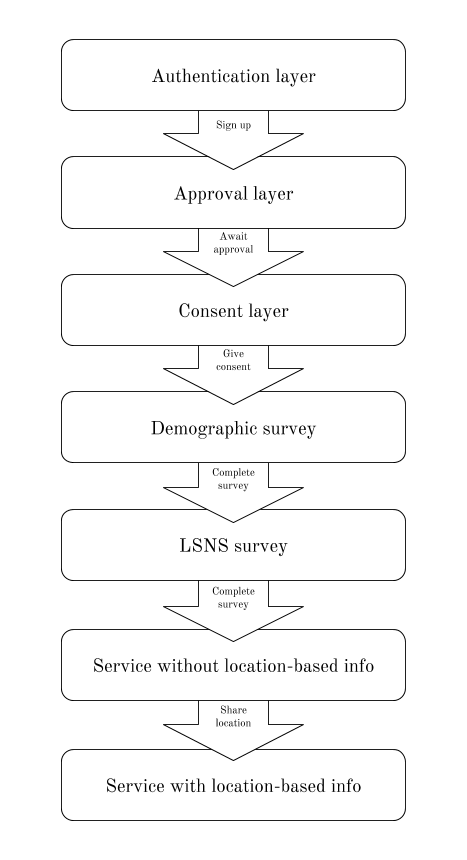
\includegraphics[scale=0.5]{images/entry_architecture.png}
  \caption{Layers of the service and the actions required to reach them}
  \label{fig:entry_architecture}
\end{figure}

\subsubsection*{Approval process}

After installing the app and signing up for an account, participants were instructed to wait for their account to be approved. We regularly checked for new sign-ups and evaluated each request to join based on past personal contact with the user, Facebook profile information if the user requested to join the study via Facebook, and in the absence of all other information, by sending the user an email requesting them to introduce themselves. Four user accounts were not approved: two because the users signed up from outside of Germany, one due to insufficient information about the person, and one that was an existing user trying to sign in with a different email address.

\subsubsection*{Welcome email}

After their account was reviewed and approved, participants were sent an email to welcome them to the user community. The welcome email also contained links to instructions on how to get started with the app, the rules of the service, and information about the study. Participants were encouraged to reach out with any questions or concerns.

\subsubsection*{Consent and Surveys}

When participants logged into the app for the first time after approval, they were taken to the in-app consent form. This form asked users to agree to contribute their data to the study and separately requested permission to log particularly sensitive location data. Forced migrant participants received extra information about the consent to address ethical concerns when working with participants from vulnerable populations.

After providing consent, participants filled out a demographic information questionnaire to give us a sense of gender, age, country-of-origin, and user group representation. They also completed the Lubben Social Network Scale (LSNS) six-item survey, a validated self-report measure of social isolation that correlates with negative health effects \cite{chang_validation_2018}. We used this survey to obtain a rough impression of the level of social isolation of our participants at the start of the study. The questions from these two surveys are listed in appendix~\ref{app:questionnaires-demographic} and appendix~\ref{app:questionnaires-lsns}. Only after providing consent and completing the two surveys were participants granted full access to the app for the duration of the study.

\subsubsection*{Passive Sampling Data Logging}
\label{sec:passive_sampling}

Passive sampling was conducted during the study by logging user updates to the system in the back-end server application. The implementation of this data logging is described in chapter~\ref{cha:prototype}. This was intended to help us understand how participants used the app.

\subsubsection*{Active Sampling Questionnaire}
\label{sec:active_sampling}

Active sampling was conducted through surveys that appeared to the user on the dashboard of the app as ``pending reviews''. The survey appeared immediately after completing an offer, the moment when freecyclers usually meet in person, and asked for a brief review of the hand-over. The intention of the active sampling was to collect data on any out-of-app interactions that occurred because of use of the freecycling system. We asked with whom, where, and how the contact was made. We also asked questions about satisfaction and likelihood of meeting up again in an attempt to measure the quality of the social contact. The exact questions of the survey can be found in appendix~\ref{app:questionnaires-review}.

% This will trigger a questionnaire in the offer recipient’s app as well. Same questions, minus the question about to whom they gave their offer. Responses will allow us to measure reduction of social isolation, by confirming successful (i.e. complete) instances of “freecycling contact”, and by giving a simplistic metric of the quality of the contact.

\subsubsection*{End-of-Study Questionnaire}

At the end of the trial, we contacted participants individually to arrange payment of the study reward and collect post-trial data. The app was removed from the Android Play Store and the back-end server was shut down to prevent continued use of the service.

% TODO: Why SUS?
We had participants fill out a questionnaire to measure the usability of the app on the System Usability Scale (SUS) (see appendix~\ref{app:questionnaires-usability}). The questionnaire also included ten additional questions with the same answer scale, loosely based on the indicators of social isolation defined by \citeA{cornwell_measuring_2009}. These were intended to provide additional data on the value of the app for reducing social isolation. See appendix~\ref{app:questionnaires-usefulness} for the full list of those questions.


\section{Analysis}

All data collected in this third phase of the study was quantitative and required no qualitative analysis. We downloaded the data from the prototype services' database as three JSON files, one for each collection. The users collection file contained all the demographic and initial social isolation measurement data. The reviews collection file contained the active sampling data, and the datapoints collection file contained the passive sampling data.

We used a Ruby script to clean up the data and convert the JSON files into CSV files. Because the number of users and reviews was small, we could analyze those data by hand, summing and averaging statistics in a spreadsheet.

The larger datapoint dataset required more automated analysis. We wrote a script in Ruby to process and summarize the results. We tallied the datapoints by action, by user, and by action and user. This allowed us to see how many people created offers, updated their profiles, adjusted the app settings, etc.

The responses to the end-of-study SUS questionnaire were analyzed based on the classification of acceptable SUS scores developed by \citeA{bangor_empirical_2008}. The responses to the questions about usefulness were considered individually.


\section{Results}

\subsubsection*{Passive Sampling Results}

Only 4 of the 23 participants posted offers in the app in total during the two-week trial, which is roughly 1 post for every 6 users. When compared with posting rates in other Münster freecycling platforms, this is abnormally frequent posting. One of the most active freecycling services in Münster had roughly 1 post for every 118 users in the same two-week period as the trial. One of the less active services saw fewer than 1 post per 1000 users. Thus, relative to the size of the community, the posting rate was very high, which indicates the potential to create many opportunities for social contact. It is also possible, however, that participants were motivated to post due to the novelty of the service and the desire to support the study. A longer trial would be required to see if the trend continued.

\subsubsection*{Active Sampling Results}

Just one participant, a forced migrant, reported actually completing an offer. This interaction was reported to be arranged over WhatsApp with a user who was not a forced migrant and took place at the participant's home. The participant reported being satisfied with the interaction and believed they were likely to contact the person again.

\subsubsection*{Usability Survey Results}

We used the System Usability Scale (SUS) to evaluate the usability of the prototype service. The average SUS score across all users was 82.6. Among forced migrant participants, the average score was 82.1 and among freecyclers it was 82.9.

\begin{figure}[ht]
  \centering
  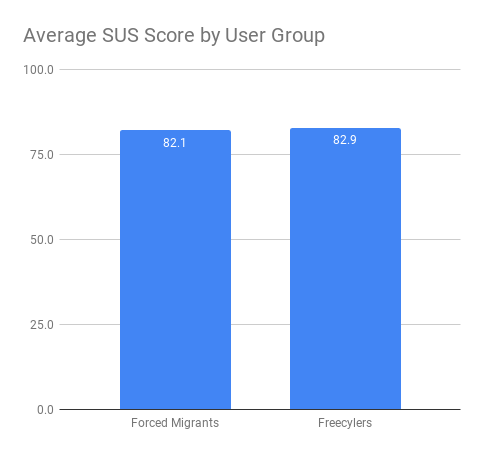
\includegraphics[scale=0.5]{images/sus_scores.png}
  \caption{Usability survey responses: user group comparison}
  \label{fig:sus_scores}
\end{figure}

\subsubsection*{Usefulness Survey Results}

In the final survey about the prototype service's potential to reduce social isolation (see appendix~\ref{app:questionnaires-usefulness}), just one participant said the service led to increased contact with others during the two-week trial: the same participant who completed an offer.

\begin{figure}[ht]
  \centering
  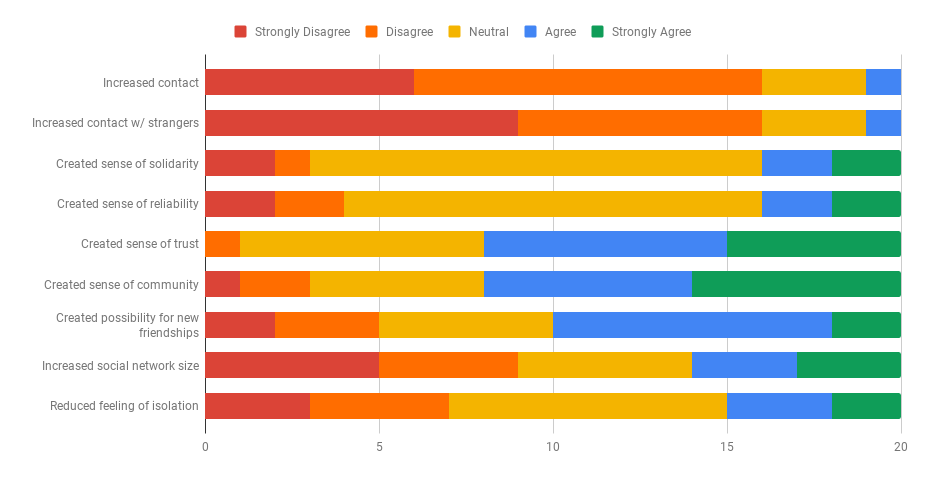
\includegraphics[scale=0.4]{images/usefulness_survey_results.png}
  \caption{Usefulness survey responses: all responses}
  \label{fig:usefulness_survey_results}
\end{figure}

A majority of the participants in both user groups disagreed or strongly disagreed with the statements ``I think using this system increased my contact with others during the last two weeks'', ``I made contact with people outside of my normal circles through this system'', and ``I think this app increased the size of my social network in Münster.''

On the other hand, a majority of the participants in both user groups agreed or strongly agreed with the statements ``I feel like part of a community while using this system'' and ``I think the contacts made through this app are likely to lead to new friendships.''

Furthermore, a majority of both user groups responded neutrally to the statements ``I feel like I have a lot in common with other people using this system'' and ``I found I could rely on the other users of this system.''

The two user groups responded oppositely to just one question, the question about social isolation. A majority of the forced migrant participants agreed with the statement ``I think this app made me feel less isolated from others in Münster'' while a majority of the freecyclers disagreed.

\begin{figure}[ht]
  \centering
  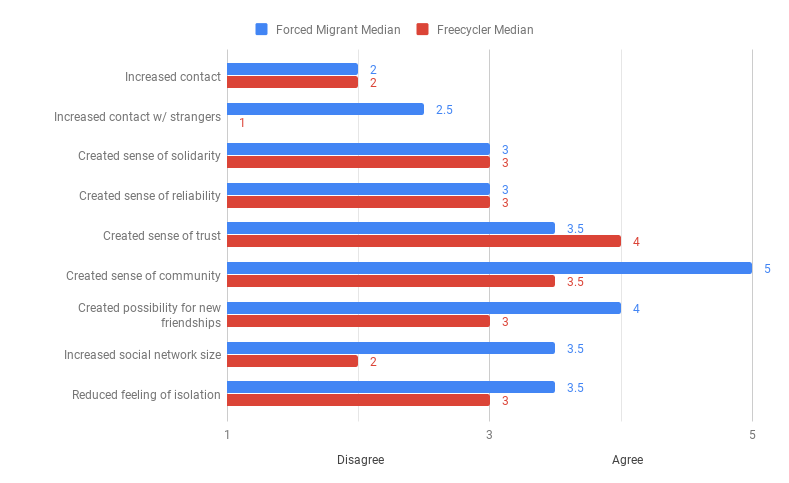
\includegraphics[scale=0.5]{images/usefulness_survey_medians.png}
  \caption{Usefulness survey responses: user group comparison}
  \label{fig:usefulness_survey_medians}
\end{figure}
